% Options for packages loaded elsewhere
\PassOptionsToPackage{unicode}{hyperref}
\PassOptionsToPackage{hyphens}{url}
%
\documentclass[
  10,
  openany]{book}
\usepackage{amsmath,amssymb}
\usepackage{iftex}
\ifPDFTeX
  \usepackage[T1]{fontenc}
  \usepackage[utf8]{inputenc}
  \usepackage{textcomp} % provide euro and other symbols
\else % if luatex or xetex
  \usepackage{unicode-math} % this also loads fontspec
  \defaultfontfeatures{Scale=MatchLowercase}
  \defaultfontfeatures[\rmfamily]{Ligatures=TeX,Scale=1}
\fi
\usepackage{lmodern}
\ifPDFTeX\else
  % xetex/luatex font selection
  \setmainfont[]{Times New Roman}
\fi
% Use upquote if available, for straight quotes in verbatim environments
\IfFileExists{upquote.sty}{\usepackage{upquote}}{}
\IfFileExists{microtype.sty}{% use microtype if available
  \usepackage[]{microtype}
  \UseMicrotypeSet[protrusion]{basicmath} % disable protrusion for tt fonts
}{}
\makeatletter
\@ifundefined{KOMAClassName}{% if non-KOMA class
  \IfFileExists{parskip.sty}{%
    \usepackage{parskip}
  }{% else
    \setlength{\parindent}{0pt}
    \setlength{\parskip}{6pt plus 2pt minus 1pt}}
}{% if KOMA class
  \KOMAoptions{parskip=half}}
\makeatother
\usepackage{xcolor}
\usepackage[left=2.54cm, right=2.54cm, top=2.54cm, bottom=2.54cm]{geometry}
\usepackage{longtable,booktabs,array}
\usepackage{calc} % for calculating minipage widths
% Correct order of tables after \paragraph or \subparagraph
\usepackage{etoolbox}
\makeatletter
\patchcmd\longtable{\par}{\if@noskipsec\mbox{}\fi\par}{}{}
\makeatother
% Allow footnotes in longtable head/foot
\IfFileExists{footnotehyper.sty}{\usepackage{footnotehyper}}{\usepackage{footnote}}
\makesavenoteenv{longtable}
\usepackage{graphicx}
\makeatletter
\def\maxwidth{\ifdim\Gin@nat@width>\linewidth\linewidth\else\Gin@nat@width\fi}
\def\maxheight{\ifdim\Gin@nat@height>\textheight\textheight\else\Gin@nat@height\fi}
\makeatother
% Scale images if necessary, so that they will not overflow the page
% margins by default, and it is still possible to overwrite the defaults
% using explicit options in \includegraphics[width, height, ...]{}
\setkeys{Gin}{width=\maxwidth,height=\maxheight,keepaspectratio}
% Set default figure placement to htbp
\makeatletter
\def\fps@figure{htbp}
\makeatother
\setlength{\emergencystretch}{3em} % prevent overfull lines
\providecommand{\tightlist}{%
  \setlength{\itemsep}{0pt}\setlength{\parskip}{0pt}}
\setcounter{secnumdepth}{5}
\ifLuaTeX
\usepackage[bidi=basic]{babel}
\else
\usepackage[bidi=default]{babel}
\fi
\babelprovide[main,import]{spanish}
\ifPDFTeX
\else
\babelfont[spanish]{rm}{Times New Roman}
\fi
% get rid of language-specific shorthands (see #6817):
\let\LanguageShortHands\languageshorthands
\def\languageshorthands#1{}
\usepackage{booktabs}
\usepackage{longtable}
\usepackage[none]{hyphenat}
\raggedbottom
\usepackage{blindtext}


\usepackage{scrlayer-scrpage}
\usepackage{lipsum}% just to generate text for the example

\pagestyle{scrheadings}
\clearpairofpagestyles
\ohead{\rightmark}
\cfoot[\pagemark]{\pagemark}



\let\oldmaketitle\maketitle
\AtBeginDocument{\let\maketitle\relax}
\usepackage{booktabs}
\usepackage{longtable}
\usepackage{array}
\usepackage{multirow}
\usepackage{wrapfig}
\usepackage{float}
\usepackage{colortbl}
\usepackage{pdflscape}
\usepackage{tabu}
\usepackage{threeparttable}
\usepackage{threeparttablex}
\usepackage[normalem]{ulem}
\usepackage{makecell}
\usepackage{xcolor}
\ifLuaTeX
  \usepackage{selnolig}  % disable illegal ligatures
\fi
\usepackage[]{natbib}
\bibliographystyle{apalike}
\IfFileExists{bookmark.sty}{\usepackage{bookmark}}{\usepackage{hyperref}}
\IfFileExists{xurl.sty}{\usepackage{xurl}}{} % add URL line breaks if available
\urlstyle{same}
\hypersetup{
  pdftitle={RECUPERACIÓN, EXTRACCIÓN Y CLASIFICACIÓN DE INFORMACIÓN DE SABER UCV},
  pdfauthor={José Miguel Avendaño Infante},
  pdflang={es-ES},
  hidelinks,
  pdfcreator={LaTeX via pandoc}}

\title{RECUPERACIÓN, EXTRACCIÓN Y CLASIFICACIÓN DE INFORMACIÓN DE SABER UCV}
\usepackage{etoolbox}
\makeatletter
\providecommand{\subtitle}[1]{% add subtitle to \maketitle
  \apptocmd{\@title}{\par {\large #1 \par}}{}{}
}
\makeatother
\subtitle{Caso de Estudio Repositorio www.saber.ucv.ve}
\author{José Miguel Avendaño Infante}
\date{2023-10-20}

\begin{document}
\maketitle

%\vspace{-2.0cm}
\pagenumbering{roman}
\begin{center}
	UNIVERSIDAD CENTRAL DE VENEZUELA\\
	FACULTAD DE CIENCIAS\\
	POSTGRADO EN CIENCIAS DE LA COMPUTACI\'ON\\

	\begin{figure}
						\centering
						  
\includegraphics[height=.7\textwidth]{images/UCV.png}
  \end{figure}
  \vspace{1.5cm}
  \large{\textbf{RECUPERACI\'ON, EXTRACCI\'ON Y CLASIFICACI\'ON DE \\ INFORMACI\'ON DE SABER UCV}}

  \vspace{3cm}
  Trabajo de grado de Maestría presentado ante la \\
  ilustre Universidad Central de Venezuela por el\\
  Econ. José Miguel Avendaño Infante para  optar
  al título de \\Magister Scientiarum en Ciencias de la Computaci\'on\\
  \vspace{0.5cm}
  Tutor: Dr. Andres Sanoja\\
  \vspace{1.5cm}
  Caracas - Venezuela\\
  Octubre 2023
\end{center}


\newpage
\thispagestyle{empty}
\large{\textbf{Resumen:}}

Se presenta una propuesta de aplicación web distribuida para implementar un Sistema de Recuperación de Información (\emph{information retrieval}) mediante técnicas de Procesamiento de Lenguaje Natural (NLP), de indexación en base de datos y visualizaciones con gráficos y gráfos de coocurrencias de palabras para los trabajos especiales de pre y postgrado realizados por los estudiantes de la Universidad Central de Venezuela que se encuentran alojados en el repositorio www.saber.ucv.ve.

Esta propuesta se basa principalmente en que mediante la búsqueda de palabras o frases se genere un (\emph{query}), y mediante la técnica conocida como "\emph{full text search}" se puedan extraer los trabajos en que se encuentran contenidas tales palabras y a partir de ahí enriquecer la experiencia del usuario con la presentación de la información recuperada.

La aplicación se diseña como un sistema distribuido en distintos contenedores soportando cada uno un proceso para el funcionamiento, teniendo entre los principales el de base de datos, el servidor de la aplicación y otro con los distintos procesamientos que son efectuados sobre los textos.

\thispagestyle{empty}


%\newpage


\setlength{\abovedisplayskip}{-5pt}
\setlength{\abovedisplayshortskip}{-5pt}
\thispagestyle{empty}

\newpage
\begin{center}
\large{\textbf{\emph{\Huge{Dedicatoria:}}}}
\end{center}
\thispagestyle{empty}
\vspace*{5cm}
\thispagestyle{empty}
\begin{center} \Large \emph{A  mi hijo Cassiel y  } \end{center}
\vspace*{1cm}
\begin{center} \Large \emph{mi esposa Waleska.} \end{center}



\newpage
\begin{center}
\large{\textbf{\emph{\Huge{Agradecimientos:}}}}
\end{center}
\thispagestyle{empty}
\vspace*{2cm}
\thispagestyle{empty}

- A mi madre, obvio, sino no habría ni una sola palabra acá.\\\\
- A mi padre Fernando por negarme el Atari e insistir en el Oddysey 2.\\\\
- A mi tía Mercedes Infante.\\\\
- A Cesar Alejandro García por todas las ayudas.\\\\
- A mi hermano David por su soporte.\\\\
-   Dr. Andres Sanoja primero por aceptar la tutoría y enseñarme qué es la investigación dentro de una comunidad científica.\\\\
-   Dr. José Mirabal por siempre andar con alguna idea a desarrollar y el tiempo dedicado a escuchar las propuestas y complementar esta Investigación.\\\\
-   Dra. Concettina Di Vasta por las imponentes sesiones de 2 horas 15 minutos llenas de coherencia y conocimiento.\\\\
-   Dra. Haydemar Nuñez por la rigurosidad al impartir los conocimientos.\\\\
-   Dra. Vanessa Leguizamo por tomarse el tiempo de revisar la solicitud de estudio de un oxidado economista y por ser mi Prof.ª.\\\\
-   Dra. Nuri Hurtado Villasana por tomarse el tiempo de escucharme y brindarme sugerencias en la elaboración de este trabajo.\\\\
-   A todo el personal del Postgrado: sus buenos días, por tener a mano la llave, por ayudar a mantener viva la Academia.\\\\
-   Mauricio Sáez Toro del equipo Saber UCV por mantener activo el Sistema Saber UCV y tener el tiempo de haber colaborado con esta investigación.\\\\
-   A toda la comunidad de creadores de software libre y open sourcem en especial a los \#useRs por motivarme a adentrarme al mundo de las ciencias de la computación.\\\\
- A Alexandra Asanovna Elbakyan, sin ella serían mínimas las citas bibliográficas de esta Investigación.






\newpage
\thispagestyle{empty}
\vspace*{5cm}
\hspace*{2cm}
\begin{quote}
Every important aspect of programming arises somewhere in the context of sorting or searching.

--- Donald Knuth, \textit{The Art of Computer Programming}, Volume 3
\end{quote}
\thispagestyle{empty}
\maketitle



{
\setcounter{tocdepth}{3}
\tableofcontents
}
\listoffigures
\listoftables
\clearpage
\pagenumbering{arabic}

\hypertarget{introduccion}{%
\chapter{Introducción}\label{introduccion}}

\hypertarget{problema}{%
\chapter{Planteamiento del Problema:}\label{problema}}

\hypertarget{propuesta-tuxe9cnica}{%
\section{Propuesta Técnica:}\label{propuesta-tuxe9cnica}}

En este Capítulo se detalla la propuesta técnica de la Solución en la sección \ref{propuestatec}. Posteriormente se indica el Objetivo General \ref{objetivogral} y los Objetivos Específicos \ref{objetivosespe} que se aspiran cubrir en el desarrollo. A continuación se muestra el esquema general de la aplicación \ref{esquemas}, junto con el esquema de funcionamiento en los contenedores \ref{contenedores} y se describe el funcionamiento de cada contenedor.

Se realiza un análisis de factibilidad en la sección \ref{factibilidad} para la implementación y se muestra un cronograma \ref{cronograma} de actividades.

\hypertarget{propuestatec}{%
\section{Propuesta Técnica:}\label{propuestatec}}

Crear una Solución que funcione como una aplicación web distribuida bajo la arquitectura cliente-servidor. Del lado del servidor se encontrarán contenedores que alojarán los distintos servicios necesarios para el funcionamiento.

Del lado del cliente se podrán formular los \emph{querys} con múltiples atributos (la frase a buscar, la jerarquía académica, intervalo de fechas, facultad y/o escuela de adscripción).

La Solución permitirá generar procesos de extracción de información (\emph{information retrieval}) y los resultados se mostrarán en tablas interactivas, gráficos y grafos de coocurrencia de palabras. Adicionalmente se indicarán recomendaciones de textos basados en la similitud que presente un documento con los otros.

Los textos del resumen de cada tesis con los cuales se conformará el \emph{Corpus}, serán obtenidos y actualizados mediante técnicas de \emph{web crawling} realizadas al repositorio Saber UCV.

Se opta por la estrategia de hacer el \emph{web crawling} a los documentos contenidos en Saber UCV al no ser posible, al momento de realizar esta propuesta, la obtención de la base de datos de los documentos ahí alojados.

La Solución propuesta está diseñada para irse actualizando periódicamente incorporando los nuevos documentos que sean alojados en el repositorio Saber UCV.

Contará con un procedimiento que permite clasificar los documentos (tesis) por área académica, según donde haya efectuado estudios el autor del trabajo, al ser la tesis el requisito necesario para obtener el título de grado. Actualmente el repositorio Saber UCV no dispone de esta clasificación.

\hypertarget{objetivogral}{%
\section{Objetivo:}\label{objetivogral}}

Crear una Solución que permita realizar la clasificación de documentos y la búsqueda de información sobre los trabajos de investigación que se encuentran en el Repositorio SABER UCV usando técnicas de extracción de información (\emph{information retrieval}).

Para el procesamiento de las búsquedas será usado un sistema distribuido con distintos componentes (contenedores) que permitan la ingesta, procesamiento y transformación de los datos, al igual que el alojamiento de los mismos en una base de datos.

\hypertarget{objetivosespe}{%
\section{Objetivos Específicos}\label{objetivosespe}}

\begin{itemize}
\item
  \emph{Querys} multi atributo en distintas dimensiones: tiempo, jerarquías (pregrado, especializaciones, maestría y/o doctorado), facultad ,carreras o postgrados.
\item
  A cada resultado que arroje la búsqueda se le debe asignar un nivel de relevancia. El conjunto de los textos recuperados se debe mostrar ordenadamente de mayor a menor relevancia. La asignación de la relevancia será hecha mediante una función que cuente con distintos parámetros.
\item
  Los datos: textos, fechas, clasificaciones, y demás que sean necesarios para el funcionamiento de la Solución, deben registrarse en una base de datos estructurada y la ingesta y consulta se efectuará mediante un manejador de base de datos.
\item
  Generar recomendaciones de textos basados en la similitud coseno que presente un documento con cada uno de otros que conforman el \emph{Corpus}.
\item
  En los documentos extraídos se debe contar con el enlace a los documentos que reposan en Saber UCV.
\item
  Permitir la concurrencia de accesos al Sistema.
\item
  La tolerancia a fallas en los contenedores.
\item
  Contar con el certificado SSL para acceso seguro por parte de los visitantes.
\item
  Procesar las coocurrencias de las palabras más comunes las cuales se deberán visualizar mediante grafos.
\item
  Disponer de una aplicación web para el acceso al Sistema por parte del cliente.
\item
  Disponer de ventanas emergentes de ayuda en la interface gráfica de la aplicación web.
\item
  En la representación de coocurrencias de palabras mediante grafos, se debe poder filtrar documentos interactivamente al hacer \emph{click} con el \emph{mouse} sobre los arcos que unen un par de nodos, donde cada uno de estos representa la coocurrencia de una dupla de palabras. El \emph{click} generará el evento para el query sobre los documentos que contienen esa determinada coocurrencia.
\end{itemize}

\hypertarget{esquemas}{%
\section{Esquema del SSCSU:}\label{esquemas}}

Se representa el Sistema y sus interacciones mediante un esquema con un elevado grado de abstracción. Ver figura \ref{fig:esquema}.

\begin{figure}
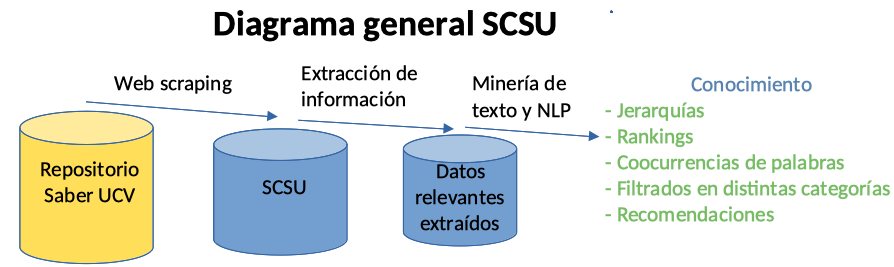
\includegraphics[width=1\linewidth]{formas/diagramageneral} \caption{Esquema General}\label{fig:esquema}
\end{figure}

En la figura \ref{fig:esquema} se muestra como el SSCSU está diseñado para que mediante técnicas de \emph{web crawling} se pueda extraer la información del repositorio Saber UCV. Posteriormente el sistema ante la consulta del usuario va a recuperar los documentos que sean relevantes, representando el conocimiento con la generación de jerarquías, rankings, coocurrencias de las palabras más mencionadas y recomendaciones de texto según similitudes.

El SSCSU se implementará mediante el uso de Docker. En la figura \ref{fig:esquemadocker} se muestra el esquema con los contenedores.

\begin{figure}
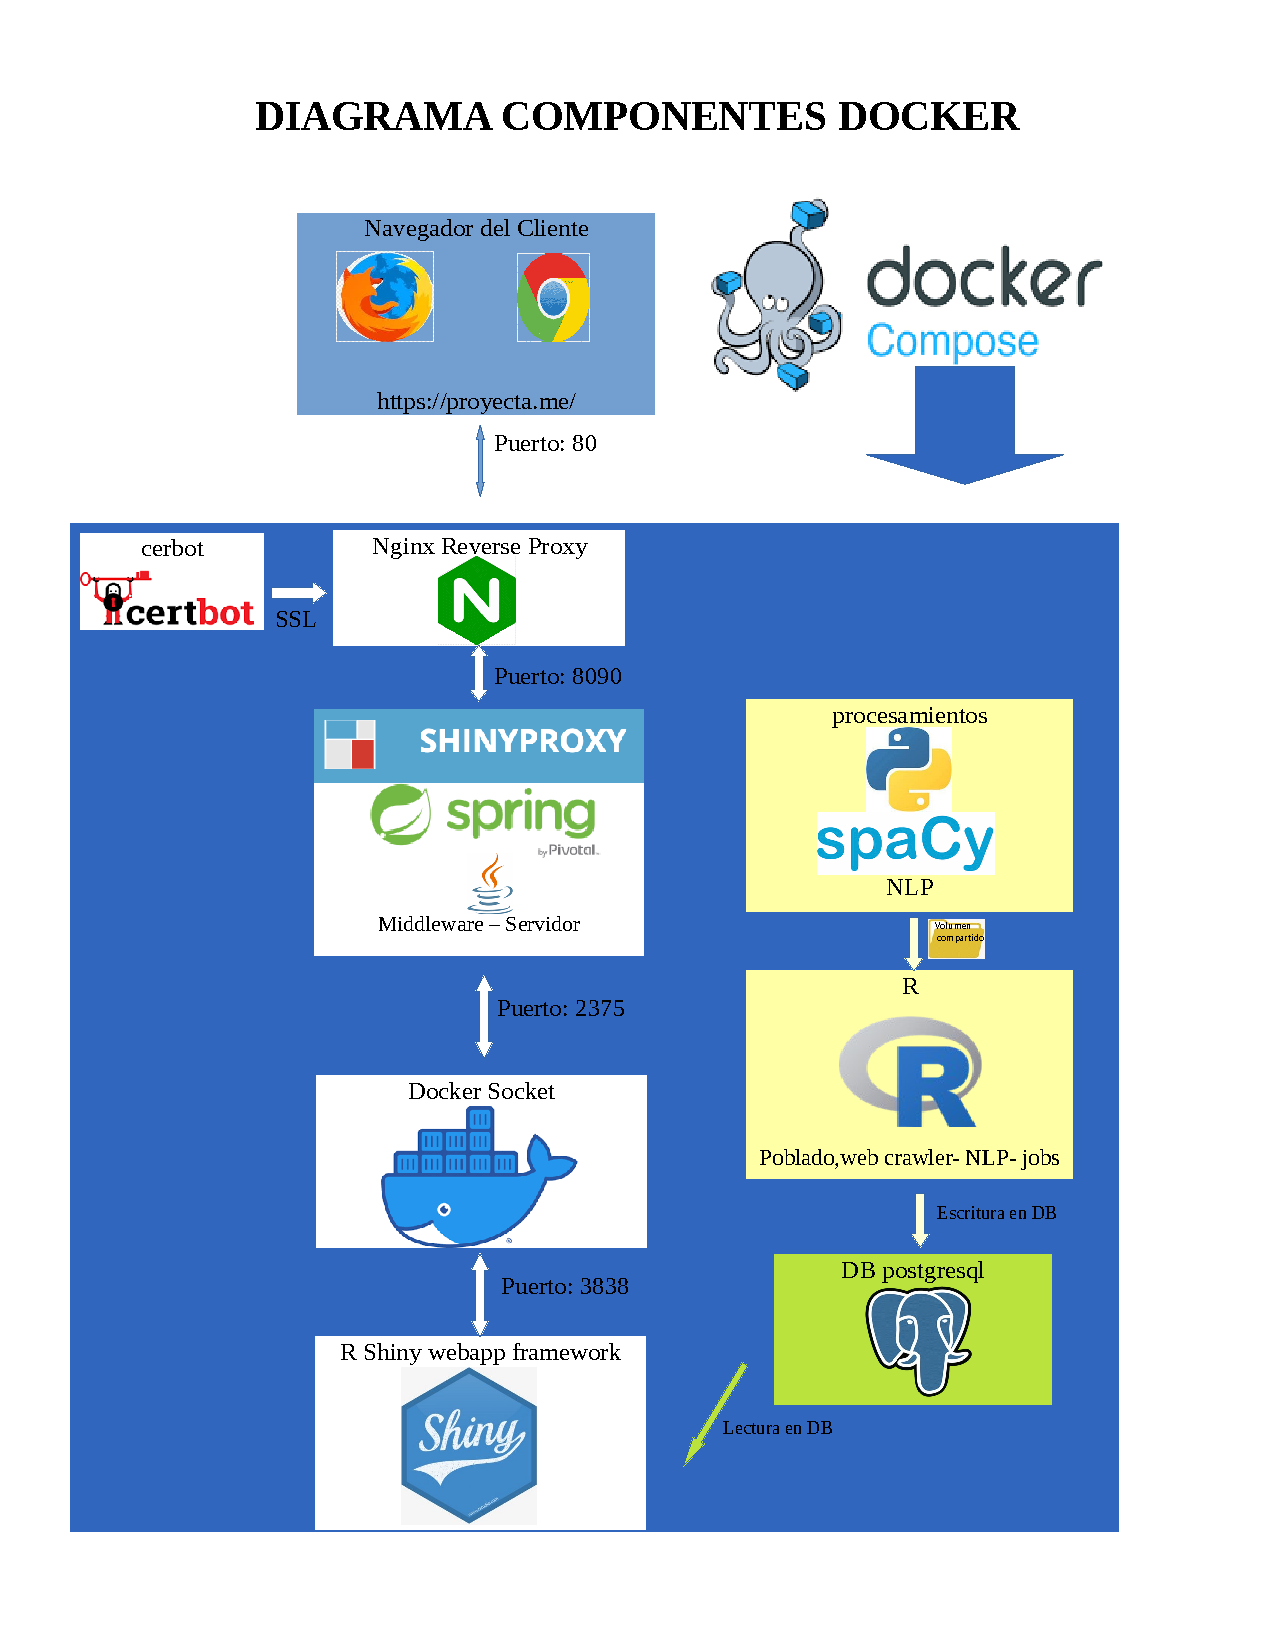
\includegraphics[width=0.9\linewidth]{formas/diagrama_docker1} \caption{Diagrama de Componentes}\label{fig:esquemadocker}
\end{figure}

\hypertarget{cliente---servidor}{%
\subsection{Cliente - Servidor:}\label{cliente---servidor}}

La arquitectura \textbf{cliente-servidor} en esta Propuesta se basa en:

\hypertarget{cliente---navegador-web}{%
\subsubsection{1 - Cliente - Navegador web:}\label{cliente---navegador-web}}

El acceso del cliente a la aplicación web se hace en el navegador web. Este realiza la petición al servidor que aloja la Solución. Actualmente se cuenta con un prototipo al que se puede acceder en la dirección \url{https://proyecta.me/}.

El sistema no está diseñado para usarse desde dispositivos móviles, aunque igualmente es viable el acceso no estando optimizada la interfaz del usuario ni las visualizaciones de los resultados de los \emph{querys}.

\hypertarget{servidor}{%
\subsubsection{2 - Servidor:}\label{servidor}}

El prototipo del sistema requiere para funcionar al menos estos recursos:

\begin{itemize}
\tightlist
\item
  2 CPU virtual
\item
  2 GB de memoria RAM
\item
  50 GB de disco duro
\end{itemize}

En el servidor se instala el software Docker sobre el cual se despliegan los siguientes contenedores:

\hypertarget{contenedores}{%
\subsection{Contenedores:}\label{contenedores}}

\hypertarget{docker-compose}{%
\subsubsection{Docker Compose:}\label{docker-compose}}

Funciona como un orquestador para correr aplicaciones distribuidas en múltiples contenedores usando un archivo en formato yml donde se establecen las imágenes, los puertos y los volúmenes que serán usados y compartidos por cada uno de los contenedores.

\hypertarget{contenedor-con-nginx}{%
\subsubsection{Contenedor con Nginx:}\label{contenedor-con-nginx}}

Es el servidor web/proxy inverso de código abierto que sirve para redireccionar las peticiones del puerto 80 al puerto 8090. Mediante este contenedor también se define el certificado SSL para permitir conexiones por el protocolo HTTPS.

Este contenedor fue generado desde una imagen oficial de NGINX que se encuentra en el \textbf{\emph{docker hub}} \footnote{repositorio de imágenes de contenedores de docker.} sin añadir ninguna capa (layer) adicional.

\hypertarget{contenedor-con-cerbot}{%
\subsubsection{Contenedor con Cerbot:}\label{contenedor-con-cerbot}}

Cerbot es una herramienta de código abierto que permite habilitar las conexiones mediante el protocolo HTTPS con el uso de un certificado ``Let´s Encrypt''. El uso de este certificado está asociado al uso de un dominio en el \emph{deploy} de la aplicación.

Este contenedor fue generado desde una imagen de CERBOT del \textbf{\emph{docker hub}} sin ninguna modificación posterior.

\hypertarget{conshinyproxy}{%
\subsubsection{Contenedor con Shinyproxy:}\label{conshinyproxy}}

Es una implementación del servidor ``\emph{Spring boo}t'' que dará servicio a las aplicación web desarrolladas en \emph{shiny} \footnote{Shiny un framework para crear aplicaciones web en el lenguaje de programación R.} \ref{conshiny}. Con el uso de este \emph{middleware} se obtienen las siguientes ventajas:

\begin{itemize}
\item
  Ante cada petición de acceso al servidor se despliega un \emph{workspace} completamente aislado, es decir, un contenedor distinto. Las aplicaciones desarrolladas en \emph{shiny} son \emph{single threaded} y adoptar esta estrategia representa una ventaja, motivado a que se pueden controlar los recursos de memoria y cpu asignados a cada contenedor que se despliega.
\item
  Permite establecer \emph{login} en el uso de la aplicación y grupos de usuarios. También da soporte a distintos métodos de autenticación. Si bien en estos momentos la aplicación es de libre acceso, en algún momento se pudiese restringir y no sería necesaria ninguna modificación en la arquitectura, más allá de cambiar el archivo de configuración.
\item
  Uso de una tecnología estable y probada.
\end{itemize}

Es necesario destacar que originalmente \emph{Shiny} como \emph{framework} cuenta con su propio software que actúa como servidor, pero para tener acceso a ciertas funcionalidades es necesario pagar por el servicio directamente a la Fundación RStudio Software y usar el alojamiento que ellos proveen, no siendo todos los componentes de código abierto. Por ejemplo, el acceso mediante \emph{login} no está disponible en la versión libre del \emph{Shiny Server} sino en la \emph{Shiny Server Professional}.

Ciertas configuraciones de librerías e incluso la propia contenerización de la aplicación, no es posible usando el servicio pago, así que la propuesta acá adoptada, si bien representa un mayor esfuerzo en la configuración, claramente implica que se obtienen una serie de ventajas, por todas las adaptaciones y control que es posible realizar al y sobre el sistema.

Este contenedor funciona en el puerto 2375 y fue generado desde la imagen del docker hub \emph{Shinyproxy} sin ninguna modificación.

\hypertarget{conshiny}{%
\subsubsection{\texorpdfstring{Contenedor con ``\emph{R Shiny Web App framework}'':}{Contenedor con ``R Shiny Web App framework'':}}\label{conshiny}}

En este contenedor es donde reposa la aplicación web con todas las librerías necesarias para generar las visualizaciones y remitir los \emph{querys} al contenedor del manejador de la base de datos \ref{conposgres} . Como comentamos anteriormente, cada vez que ocurre desde el navegador del cliente una petición de acceso, desde el contenedor \emph{shinyproxy} \ref{conshinyproxy}, se crea una replica de este contenedor con todos los elementos necesarios para que la app funcione correctamente.

En caso de presentar alguna falla, el sistema sería tolerante, porque se pueden seguir recibiendo peticiones que replicarían una imagen nueva del contenedor sin afectar al que presentase el fallo, o viceversa.

Desde este contenedor se realiza el acceso de lectura al contenedor que contiene \emph{PostgreSQL} \ref{conposgres} donde reposa la base de datos que contiene los textos ya procesados.

Por los momentos no hay escritura de datos en las tablas, pero está contemplado que se registren los querys formulados en alguna tabla, junto con los documentos que el usuario revisa mediante las interacciones, para así generar métricas de calidad del sistema y del uso que se le da.

La imagen que se usa en este servidor fue definida a medida con todos los recursos necesarios.

En un posterior Capítulo a desarrollar en donde se mostrará el proceso de desarrollo de la Solución, serán descritas todas las librerías que se encuentran incluidas en este contenedor y se expondrán las razones para seleccionar cada una de ellas.

Varios de los procesos que se ejecutan en este contenedor ocurren al momento de recibir un \emph{query,} no obstante todos los procesos que puedan ser pre computados, se trata de ejecutarlos previamente en el contenedor ``R Servicios'' \ref{conservicios}, para lograr así la disminución de los tiempos.

Funcionalidades principales: \textbf{ENTRADAS}

\begin{itemize}
\item
  Contiene un campo para la entrada de texto que generará el query.
\item
  Contiene un selector para indicar si se quiere generar la coocurrencia de palabras
\item
  Contiene tablas para seleccionar:

  \begin{enumerate}
  \def\labelenumi{\arabic{enumi})}
  \tightlist
  \item
    Nivel académico del trabajo. Opciones (pregrado, especialización, maestría, doctorado).
  \item
    Facultad o Centro de adscripción. Opciones: 11 Facultades más un centro (CENDES).
  \item
    Nombre del pregrado o postgrado. En total son 412 las opciones.
  \end{enumerate}

  Cada una de las tablas anteriores se actualiza según se vayan seleccionando las relaciones y la disponibilidades. Por ejemplo, al seleccionar pregrado solo se mostrarán los nombres de las carreras de pregrado, pero si se selecciona también el nombre de la Facultad, sólo se mostrarán las carreras de pregrado dentro de la Facultad seleccionada. Para una determinada tabla también se permiten selecciones múltiples dando una total flexibilidad al momento de ejecutar los \emph{querys}.
\end{itemize}

\textbf{SALIDAS} - Ante el \emph{query} se genera:

\begin{itemize}
\item
  Una tabla creada con la librería \emph{reactable}. En la misma se muestra cada uno de los documentos recuperados con los distintos atributos disponibles: autor, fecha, palabras clave, texto resumen. El orden en que aparece está generado con una función de ranking. Adicionalmente se muestra un enlace al repositorio Saber UCV que es donde se encuentra alojado el respectivo trabajo (el documento en PDF). Igualmente se presentan los textos que tienen mayor similitud con el texto seleccionado.
\item
  Un gráfico con la frecuencia por año de los trabajos extraídos mediante el \emph{query}. El gráfico se generá con la librería \emph{apexcharter} que es un wraper para Javascript, por lo cual el gráfico tiene ciertas interactividades. Con el \emph{hoover} muestra el valor de cada columna.
\item
  Gráfico de coocurrencia interactivo de palabras: se genera mediante la librería de \emph{VisNetwork} que también es un \emph{wrapper} de javascript. Este gráfico permite seleccionar un arco de unión entre dos palabras coocurrentes. Al realizar la selección se filtran un subconjunto de los documentos que contienen ambas palabras representadas por nodos. Los documentos filtrados se mostrarán en una tabla contigua, también generada en \emph{reactable}, donde sólo se incluye el texto resumen de cada trabajo. En un próximo Capítulo a desarrollar será mencionado el diseño y funcionamiento a detalle de esta visualización.
\item
  Gráfico de coocurrencia estático de palabras: mediante la librería \emph{ggraph} son generados un par de gráficos con distintas granularidades. El primero exhibe la misma coocurrencia de palabras expuesta en el punto anterior pero esta vez es generada en una visualización estática. En cuandoa la granularidad se muestran las palabras que coocurren dentro de todo el resumen, El segundo gráfico también muestra la coocurrencia, pero solo de palabras que coocurren una seguida de otra dentro del texto resumen, es decir que se muestran los resultados con una menor granularidad.
\end{itemize}

Con la librería \emph{UdPipe} se generan las estructuras de datos necesarias para generar los grafos (arcos y nodos).

\hypertarget{conposgres}{%
\subsubsection{Contenedor con PostgreSQL:}\label{conposgres}}

En este contenedor se tiene una imagen de \emph{PostgreSQL} versión 13.3. No fue realizada ninguna otra modificación distinta a la definición de usuarios y poblado desde base de datos incluyendo un volumen compartido para garantizar que tengamos ``datos persistentes. Este contenedor recibe consultas del contenedor''R Shiny Web App framework'' \ref{conshiny} y escritura desde el contenedor ``R imagen Servicios'' \ref{conservicios}.

En este contenedor ocurre la indexación de la base de datos y la generación del ranking al procesar el resultado con la función de PosgreSQL llamada tsrank \footnote{esta función mide la relevancia de los documentos para una consulta en particular, de modo que cuando haya muchas coincidencias, las más relevantes puedan mostrarse primero tomando en cuenta la información léxica, de proximidad y estructural del documento (título, cuerpo del documento, etc).}.

En una tabla se encuentra la identificación del documento, la fecha de creación y propiamente los textos que mediante el Tsvector \footnote{El Tsvector es una función de postgresql que crea una estructura de datos que es una lista ordenada de distintos lexemas, que son palabras que se han normalizado para fusionar diferentes variantes de la misma palabra mediante el algoritmo de Porter.} almacena el título, el resumen, el autor y las palabras clave.

En otra tabla se encuentra el almacenamiento del procesamiento que se le hace a los textos, clasificando cada una de las palabras mediante el \emph{part of speach} , y registrando el identificador del documento al que está asociada y el lema \footnote{El lema es la forma que por convenio se acepta como representante de todas las formas flexionadas de una misma palabra.}de cada una.

El TSvector es la estructura de datos que permite la búsqueda de texto completa (\emph{Full Text Seach}) mediante la función de \emph{PostgreSQL} denominada \emph{tsquery}. En un futuro capítulo a desarrollar será mostrado el diseño de las tablas con sus campos.

\hypertarget{conservicios}{%
\subsubsection{Contenedor con ``R Imagen Servicios'':}\label{conservicios}}

En este contenedor se creó una imagen con todos los servicios necesarios para realizar el web crawling, el procesamientos de textos y la descarga de los archivos desde Saber UCV para realizar la clasificación de las Tesis. Al iniciar el Sistema también contiene las funcionalidades que permiten realizar la creación de la base de datos, de las tablas y el poblado de estas.

Periodicamente es invocado este contenedor para realizar los procesos de incorporación de aquellos documentos nuevos que se detecte que están disponibles en Saber UCV.

En una primera fase se uso la utilidad del sistema operativo linux para la programación de actividades, sin embargo se está implementando el uso de la tecnología \emph{Apache Airflow} para la ejecución de la programación de los flujos de trabajo.

La imagen base usada es la del proyecto \textbf{\emph{Rocker}} {[}@RJ-2017-065:2017{]} ,la cual es una versión ampliamente probada y optimizada en, y por, la comunidad de usuarios de R.

Posteriormente serán descritas todas las librerías que fueron añadidas mediante una capa (layer) a este contenedor. Por los momentos se especifican que se encuentran agregadas las siguientes:

\hypertarget{text-mining-y-nlp}{%
\paragraph{Text Mining y NLP:}\label{text-mining-y-nlp}}

Generalmente las distintas librerías que permiten realizar procesos de \emph{Natural Language Processing} también hacen procesos de \emph{Text Mining} parcial o totalmente. En la investigación fueron evaluadas múltiples librerías como \emph{Spacy, Quanteda, OPENLP, CoreNLP, Freeling y Udpipe}.

En una futura entrega se hará una breve mención a cada una y la razón por la cual se adoptó Spacy para varios de los procesos de NLP.

Para ejecutar \emph{Spacy} es necesario usar los archivos que se encuentran en el contenedor \emph{``Python Spacy''} , \ref{conspacy} donde está instalada la libraría \emph{Spacy} que corre en \emph{Python}.

Procesos que se ejecutan llamando al contenedor ``Python Spacy'': Tokenización, POS y Lematización.

También en este contenedor se realizan los siguientes procesos:

\begin{enumerate}
\def\labelenumi{\arabic{enumi}.}
\item
  Poblado base de datos: se hace el \emph{web crawling} para el poblado inicial y adicionales de la base de dato, con los textos de los Resúmenes.
\item
  Clasificación de los documentos: mediante una rutina compuesta por varios algoritmos serán clasificados los distintos trabajos según lo antes expuesto.
\item
  Cálculo de la Similitud de los documentos: cuando se ha realizado la lematización de las palabras se procede a generar una matriz de tipo Td-Idf (term document- inverse document frecuency), que sirve de insumo para el cálculo de similitud entre los documentos. Este cálculo de similitud se realiza con la librería Quanteda.texstats y se usa la medida de similitud coseno, ya que varios autores la sitúan como una de las mejores formas de comparar la similitud entre un documento y otro.
\end{enumerate}

\hypertarget{conspacy}{%
\subsubsection{Contenedor con ``Python Spacy'':}\label{conspacy}}

Se creó una imagen que contiene un ubuntu con python, spacy y el modelo de Spacy \href{https://spacy.io/models/es\#es_core_news_sm}{es\_core\_news\_sm} . Su función es que mediante un volumen compartido pueda ser invocado desde el contenedor ``R Imagen Servicios'' \ref{conservicios} para así realizar los procesamientos de NLP antes descritos.

\hypertarget{factibilidad}{%
\section{Factibilidad:}\label{factibilidad}}

Para la propuesta del SCSU se hizo una evaluación de la factibilidad del desarrollo del proyecto que consistió en hacer pruebas de \textbf{\emph{web crawling}} sobre el repositorio Saber UCV al no ser viable la obtención del conjunto de datos por otro medio. Igualmente se realizaron pruebas sobre el hardware disponible con arquitecturas similares a la que se propondrá más adelante en nuestro desarrollo.

Estas pruebas fueron exitosas por lo cual no se estima que exista algún factor que impida la implementación del Sistema acá expuesto.

\hypertarget{teorico}{%
\chapter{Marco teórico-referencial:}\label{teorico}}

En este Capítulo se muestra el marco teórico en que se sustentan los aspectos de mayor relevancia para el desarrollo de la Solución. Principalmente se enuncian una serie de conceptos que involucran algoritmos de búsqueda, la recuperación de información, la minería de texto, el procesamiento del lenguaje natural, la estructuración de la base de datos y lo referente a la arquitectura distribuida en que se soporta la SSCSU.

\hypertarget{alghist}{%
\section{Reseña histórica:}\label{alghist}}

El profesor Donald Knuth señala, dentro del campo de las ciencias de la computación, que la \textbf{búsqueda} \emph{es el proceso de recolectar información que se encuentra en la memoria del computador de la forma más rápida posible, esto cuando tenemos una cantidad N de registros y nuestro problema es encontrar el registro apropiado de acuerdo a un criterio de búsqueda} \citep{knuth1997} (p.~392) .

Iniciamos con esta cita porque la recuperación de información gira en torno a un problema central de las ciencias de la computación que es la \textbf{búsqueda}. A continuación se mencionarán una serie de algoritmos que abordan este problema, no necesariamente resultando óptimos para dar solución a lo planteado en \ref{p2}.

En la década de 1940 cuando aparecieron las computadoras, las búsquedas no representaban mayor problema debido a que estas máquinas disponían de poca memoria \emph{RAM} pudiendo almacenar sólo moderadas cantidades de datos. Ellas estaban diseñadas para realizar cómputos y arrojar los resultados más no para tenerlos almacenados en memoria.

No obstante con el desarrollo del almacenamiento en memoria \emph{RAM} o en dispositivos de almacenamiento permanentemente, ya en la década de 1950 empezaron a aparecer los problemas de \textbf{búsqueda} y los primeras investigaciones para afrontarla. En la década de 1960 se adoptan por ejemplo estrategias basadas en arboles.

Los primeros algoritmos que sirvieron para localizar la aparición de una frase dentro de un texto, o expresado de forma más abstracta, como la detección de una subcadena \emph{P} dentro de otra cadena \emph{T}, fueron los algoritmos de \emph{Pattern-Matching} \citep{goodrich2013} (p.~584).

Así nos encontramos en la literatura con el algoritmo \emph{Fuerza Bruta} donde dado un texto T y una subcadena P, se va recorriendo cada elemento de la cadena T para detectar la aparición de la subcadena P. Si bien este algoritmo no presentaba el mejor desempeño, por contar con ciclos anestados en su ejecución, creó una forma válida de enfrentar el problema de la búsqueda de subcadenas de texto.

El algoritmo \emph{Knuth-Morris-Pratt} que se introdujo en 1976 tenía como novedad que se agregó una función que iba almacenando ``previas coincidencias parciales'' en lo que eran fallos previos y así al realizar un desplazamiento tomaba en cuenta cuántos caracteres se podían reusar. De esta forma se logró considerablemente mejorar el rendimiento en los tiempos de ejecución de \emph{O(n+m)} que son asintóticamente óptimos.

Posteriormente en 1977 el problema se enfrenta con un nuevo algoritmo que es el de \emph{Boyer-Moore} en el cual se implementan dos heurísticas (\emph{looking-glass y} \emph{character-Jump)} que permiten ir realizando algunos saltos en la búsqueda, ante la no coincidencia de la subcadena con la cadena y adicionalmente, el orden en el que se va realizando la comparación se invierte. Estas modificaciones permitieron obtener un mejor desempeño.

Sobre una modificación al algoritmo \emph{Boyer-Moore} se sustenta la utilidad \emph{grep} de la línea de comandos UNIX que igualmente le da soporte a diversos lenguajes que la usan para ejecutar búsquedas de texto con un proceso que comúnmente es conocido como \emph{grepping}. Esta utilidad fue ampliamente usada para resolver parcialmente lo expuesto en \ref{clasificacion}.

Los algoritmos mencionados anteriormente pueden ser usados en procesos de recuperación de información en conjunto con técnicas que pueden mejorar considerablemente los tiempos en la ejecución de las rutinas siendo una de estas el preprocesamiento de los textos, \emph{eg}. remover determinados caracteres, aplicar el algoritmo de porter, entre otras más.

Una estrategia que surgió para enfrentar las búsquedas de texto, fue el uso de la programación lineal donde bajo la premisa \emph{divida et impera} los problemas que requieren tiempo exponencial para ser resueltos son descompuestos en polinomios y por lo tanto se disminuye la complejidad en tiempo para ser resueltos. Entre este tipo de algoritmos se puede mencionar los de \emph{alineación del ADN .} Originalmente el algoritmo se desarrolló para resolver problemas de alineación de cadenas de ADN de forma parcial o total dentro de una cadena mayor. Posteriormente se identificó que este tipo de procedimiento era extrapolable a los subcadenas de texto. Una de las versiones de estos algoritmos es la denominada \textbf{\emph{Smith-Waterman}} que resultó de gran utilidad para resolver el problema planteado en \ref{clasificacion} ya que la estrategia de usar la utilidad \emph{grep} fue infructuosa en algunos casos.

Un gran paso para aproximarnos a la aparición de los Sistemas de Recuperación de Información lo representó el enfoque que presentan los algoritmos \emph{Tries}. Este nombre proviene del proceso de \emph{Information Retrieval} y principalmente se basa en hacer una serie de preprocesamientos a los textos para que al momento de ejecutar la búsqueda de texto, es decir, de la subcadena dentro de la cadena, ya tengamos una parte del trabajo realizado previamente y no tener que ejecutarlo todo \emph{``on the fly''}, es decir, sobre la marcha.

Un \emph{Trie} \citep{fredkin1960} es una estructura de datos que se crea para almacenar textos para así poder ejecutar más rápido la coincidencia en la búsqueda. En la propuesta de la SSCSU todos los textos van siendo procesados con distintas técnicas a medida que son insertados en la base de datos. Esto claramente representa una mejora en el desempeño con la disminución en los tiempos de búsqueda.

\hypertarget{infret}{%
\section{Recuperación de Información:}\label{infret}}

El eje central sobre el cual gira el proceso de recuperación de información (RI) es satisfacer las necesidades de información relevante que sean expresadas por un usuario mediante una consulta (\textbf{\emph{query}}) de texto. El investigador Charu Aggarwal en su libro sobre Minería de Texto \citep{miningt2012} (p.14) menciona que el objetivo del proceso de RI es conectar la información correcta, con los usuarios correctos en el momento correcto, mientras que otro de los autores con mayor dominio sobre el tema, Christopher Manning en su libro \emph{Information Retrieval} indica que ``es el proceso de encontrar materiales (generalmente documentos) de una naturaleza no estructurada (generalmente texto) que satisface una necesidad de información dentro de grandes colecciones (normalmente almacenada en computadores)'' \citep{manning2008} (p.~25).

Satisfacer una necesidad de recuperación de información no sólo se circunscribe a un problema \textbf{búsqueda} de un texto dentro de un \emph{corpus}. En la mayoría de los casos se deberá cumplir con ciertos criterios, o restricciones, como por ejemplo que el \emph{query} esté dentro de un período de fechas, o que se encuentre comprendido en un subconjunto del corpus que es a lo que se denomina \textbf{búsqueda múlti atributo}.

La información que se recolecte en una búsqueda tendrá distintos aspectos que aportarán peso en el orden en que sea presentada al usuario y no sólo vendrá dado por la aparición de las palabras sino también por otros elementos como lo puede ser la aparición de la frase del \textbf{\emph{query}} dentro del título, la proximidad (la cercanía entre dos palabras) que tengan los términos que conforman el \emph{query} o por otra parte la frecuencia que una palabra, o varias, se repitan dentro un determinado documento que compone el \emph{corpus}. Igual puede aportar un peso mayor a la recuperación de un documento las referencias (citas) que contengan otros documentos a ese determinado documento. El fin último será la extracción de los documentos que resulten de mayor relevancia para el usuario.

Incluso es válido incorporar documentos, en los resultados que arroje la búsqueda, que propiamente no coincidan con los términos buscados sino que contengan términos que sean sinónimos o también añadiendo a los resultados documentos que presenten alguna similitud con el texto del \textbf{\emph{query}}. Lo que acabamos de mencionar incorporará formalmente dentro del proceso de extracción de información algo de imprecisión con la intención última de enriquecer el proceso de \textbf{\emph{Information Retrieval}} \citep{kraft2017}.

Evaluando el proceso con cierto nivel de abstracción se tiene que el proceso de recuperación de información está compuesto principalmente por: un \emph{query}, por un corpus y por una función de \emph{ranking} para ordenar los documentos recuperados de mayor importancia a menor.

El desarrollo de los algoritmos expuestos en \ref{alghist} sumado a la necesidad de resolver los problemas asociados a la búsqueda de un texto dentro de un \emph{corpus} con múltiples atributos en tiempos aceptables y la abundante cantidad de información digital, potenciada por el uso generalizado de los computadores, abonó las condiciones para la creación de los \textbf{Sistemas de Recuperación de Información}.

\hypertarget{SRI}{%
\section{Sistemas de Recuperación de Información (SRI) :}\label{SRI}}

Los Sistemas de Recuperación de Información (\emph{Information Retrieval Systems-IRS}) son los dispositivo (software y/o hardware) que median entre un potencial usuario que requiere información y la colección de documentos que puede contener la información solicitada \citep{kraft2017} 1. El SRI se encargará de la representación, el almacenamiento y el acceso a los datos que estén estructurados y se tendrá presente que las búsquedas que sobre él recaigan tendrán distintos costos siendo uno de estos el tiempo que tarde en efectuarse.

Es de nuestro conocimiento que generalmente los datos estructurados son gestionados mediante un sistema de base de datos pero en el caso de los textos estos se gestionan por medio de un motor de búsqueda motivado a que los textos en un estado crudo carecen de estructura \citep{miningt2012} (p.~2). Son los motores de búsqueda (\emph{search engines}) los que permiten que un usuario pueda encontrar fácilmente la información que resulte de utilidad mediante un \emph{query}.

El SSCSU está diseñado como un IRS donde se pueden ejecutar querys que son procesados y los resultados que se obtienen son sometidos a una función de ranking que será expuesta en una fase posterior del desarrollo de esta investigación.

\hypertarget{ejemplos-de-irs}{%
\section{Ejemplos de IRS:}\label{ejemplos-de-irs}}

Profundizando en el tema de esta Investigación se mencionan un par de páginas de internet que funcionan coomo IRS.

\begin{enumerate}
\def\labelenumi{\arabic{enumi}.}
\item
  Una es el proyecto denominado Arvix alojado en \url{https://arxiv.org/}, que es un repositorio de trabajos de investigación. Al momento del usuario hacer un requerimiento de información, adicional al texto de la búsqueda, se pueden indicar distintos filtros a aplicar como puede ser el área del conocimiento (física, matemática, computación, etc.). Igualmente se puede indicar si se quiere buscar sólo dentro del título de una investigación, o el autor, en el \emph{abstract, o} en las referencias, por ejemplo.

  Al ejecutar una búsqueda pueden ser recuperados miles de documentos y la interacción con el sistema permite ver que se genera un \emph{ranking} en la exhibición de los resultados obtenidos. El primero de estos \emph{rankings} se ordena con base en la fecha de publicación, pero es viable que se ordenaran los documentos por la relevancia que presentan.
\item
  También está el portal de la \emph{Asociation Computery Machine} (ACM) que incorpora motores de búsqueda con particulares características facilitando la labor de investigación y extracción de información ante una determinada necesidad. Esto lo decimos porque los resultados de una búsqueda son acompañados de distintas representaciones gráficas que le dan un valor adicional a la representación de los resultados. En la figura \ref{fig:busquedasacm} se ve una de estas representaciones que incluye la frecuencia de aparición del \emph{query} en el tiempo.
\end{enumerate}

\begin{figure}

{\centering 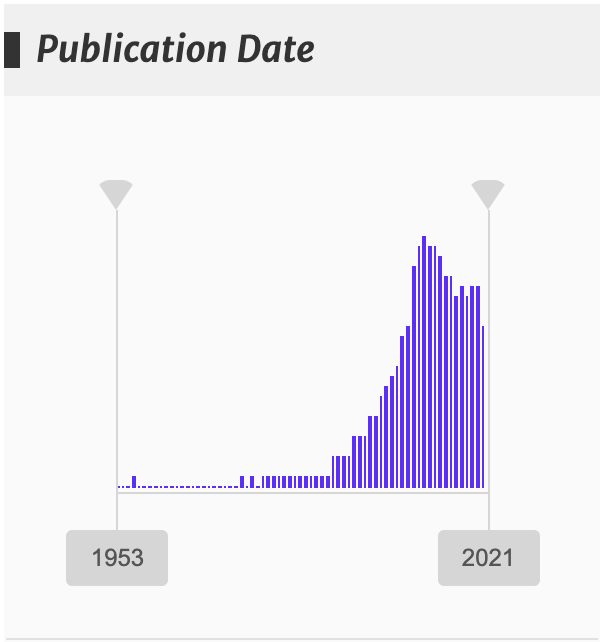
\includegraphics[width=0.4\linewidth]{images/03-marco-teorico/busquedaacm} 

}

\caption{Gráfico que acompaña resultados de búsqueda de un término en la biblioteca digital de la Association for Computing Machinery (https://dl.acm.org/)}\label{fig:busquedasacm}
\end{figure}

\hypertarget{modelos-de-recuperaciuxf3n-de-informaciuxf3n}{%
\section{Modelos de Recuperación de Información:}\label{modelos-de-recuperaciuxf3n-de-informaciuxf3n}}

\hypertarget{recuperaciuxf3n-boleana}{%
\subsection{Recuperación boleana:}\label{recuperaciuxf3n-boleana}}

Ante una búsqueda de información se recorre linealmente todo el documento para retornar un valor boleano indicando la presencia o no del término buscado. Es uno de los primeros modelos que se uso y está asociado a técnicas de \emph{grepping} \citep{manning2008} (p.3). El desarrollo de este modelo apareció entre 1960 y 1970.

El usuario final obtendrá como respuesta a su \emph{query} sólo aquellos textos que contengan el término. Es un modelo muy cercano a los típicos \emph{querys} de bases de datos con el uso de operadores ``AND'', ``OR'' y ``NOT''. En el procesamiento de los textos se genera una matriz de incidencia binaria término-documento, donde cada término que conforma el vocabulario, ocupa una fila \emph{i} de la matriz mientras que cada columna \emph{j} se asocia a un documento. La presencia de el término \emph{i} en el documento \emph{j} se denotará con un valor verdadero o un ``\textbf{1}''.

La recuperación boleana si bien representa una buena aproximación a la generación de \emph{querys} más rápidos, presenta una gran desventaja y es que al crecer la cantidad de documentos y el vocabulario, se obtiene una matriz dispersa de una alta dimensionalidad que hace poco efectiva su implementación.

Los documentos y los \emph{querys} son vistos como conjuntos de términos indexados, que luego fueron llamados ``bolsa de términos'' \emph{(bag of terms)}. Las deficiencias de este modelo recaen en que los resultados, no tienen ningún ranking. Si por ejemplo el término sobre el cual se realiza el \emph{query} aparece 100 veces en un documento y en otro aparece sólo una vez, en la presentación de los resultados ambos documentos aparecerán al mismo nivel, no pudiendo mostrar preferencia del uno sobre el otro.

Otra de las desventajas es que no se registra el contexto semántico de las palabras, incluso se pierde el orden en que aparecen las palabras en cada texto.

Este modelo se presume que en el cual se basa la implementación de Saber UCV y por eso es que en general se termina presentando el problema de que al usar el operador \emph{AND} en las búsquedas exactas mencionadas en \ref{query} se obtiene una alta \textbf{\emph{precision}} \footnote{Precision: la fracción, o porcentaje, de los documentos recuperados que son relevantes en la búsqueda efectuada.} en los resultados pero un bajo \textbf{\emph{recall}} \footnote{Recall: la fracción, o porcentaje, de los documentos relevantes en la colección que fueron recuperados por el sistema.} mientras que al usar el operador \emph{OR} da una baja \textbf{\emph{precisión}} y un gran \textbf{\emph{recall}}.

Con la propuesta del SSBSU se quiere una versión de recuperación de información que aplica métodos de mayor eficiencia, que permiten mejorar el desempeño (tiempo) y la calidad de los resultados.

\hypertarget{invind}{%
\subsection{Índices Invertidos:}\label{invind}}

Se denominan índices invertidos porque en vez de guardar los documentos con las palabras que en ellos aparecen, en estos se procede a guardar cada palabra y se indica los documentos en los cuales se encuentra y adicionalmente se puede registrar la posición en que aparece cada palabra con distintas granularidades, pudiendo ser estas: dentro del documento, del capítulo, del párrafo o de la oración. También pueden contener la frecuencia con que se presenta determinada palabra. Toda esta información nos permite mejorar los tiempos de búsqueda pero con ciertos costos.

El primero es el espacio en disco que implica guardar estos datos adicionales, que puede oscilar del 5\% al 100\% del valor inicial de almacenamiento, mientras que el segundo costo lo representa el esfuerzo computacional de actualizarlos una vez que se incorporan nuevos documentos \citep{Mahapatra2011}.

Existen diversos tipos de \textbf{Índices Invertidos} y constantemente se están realizando investigaciones que permitan mejorar su desempeño motivado en que sobre ellos recae gran parte de la efectividad que podamos obtener ejecutando los \emph{querys}. Algunos ejemplos de estos índices son el \emph{Generalized Inverted Index} (GIN), también está el RUM \footnote{En el vínculo \url{https://github.com/postgrespro/rum} se tiene acceso a la explicación e implementación de este índice para PostgreSQL.} o el VODKA \footnote{este índice fue presentado en la Postgres Conference en el año 2014 \url{https://www.pgcon.org/2014/schedule/attachments/318_pgcon-2014-vodka.pdf}}que es otra implementación con menos literatura sobre posibles usos pero con métodos disponibles para su uso en manejadores de base de datos como PostgreSQL.

El espacio que ocupa la implementación de estos índices se puede ver afectado, por un lado se tiene que se puede reducir mediante el preprocesamiento que hagamos a las palabras buscando su raiz con el stemming \{\#steaming\} o removiendo las stop words (las palabras que no generan mayor valor semántico como: la, el, tu).

Por otra parte el peso total se puede incrementar a medida que decidamos tener una granularidad más fina en el registro de las palabras y su ubicación dentro de los documentos. En el transcurso del desarrollo de nuestra investigación se indicará en cuánto se incremento el espacio de almacenamiento en disco con la aplicación de este índice y la granularidad que se adoptó junto con el valor del costo en espacio de almacenamiento.

Continuando con los índices inversos hay estrategias que significan la adopción de generar dos índices inversos para un sistema, conteniendo uno de estos la lista de documentos y la frecuencia de la palabra, mientras que el otro registra la lista con las posiciones de la palabra.

El uso de los índices invertidos permite la denominada ``búsqueda de texto completa'' (\emph{full text search}) que es uno de los pilares que sustenta a los motores de búsqueda y se entiende por este tipo de búsqueda aquella que permite encontrar documentos que contienen las palabras clave o frases determinadas en el texto del \emph{query}. Adicionalmente se puede introducir el criterio de búsqueda de texto aproximado \emph{(approximate text searching)}, que permite flexibilizar la coincidencia entre el texto requerido y el resultado.

En la Solución que se propone, la optimización en la generación de este índice quedará bajo la administración del propio manejador de base de datos que es \emph{postgreSQL}.

Cuando la base de datos que registra el índice invertido crece y no es viable almacenarla en un único computador, es necesario acudir al uso de técnicas que permitan distribuir la base de datos con el uso de tecnologías como \emph{Spark, Hadoop, Apache Storm} entre otras.

\hypertarget{rank}{%
\subsection{Scoring Model:}\label{rank}}

Es un modelo aplicado en amplias colecciones de documentos donde es necesario exclusivamente mostrar al usuario que realizó la búsqueda, una fracción de los documentos encontrados, pero es necesario que estos sean los de mayor puntuación (\emph{score}), de acuerdo a distintos criterios que permitan determinar cuales son los que tienen mayor relevancia, como lo puede ser la cantidad de veces que se repite una palabra aparecida en el \emph{query} dentro del documento, o la distancia de aparición de cada una de las palabras que conforman el query (cantidad de palabras que median entre una y otra).

También se puede asignar un peso mayor en la generación del ranking, si una, o varias, de las palabras que generan el \emph{query} aparece dentro del título, o en otros campos que se registrasen en la base de datos.

\hypertarget{procesamientos-de-texto}{%
\section{Procesamientos de texto:}\label{procesamientos-de-texto}}

En esta sección mostramos métodos de trabajo con los textos. Para el idioma español no son de abundante literatura, a diferencia de aquellos que están en el idioma inglés. Incluso hasta hace unos pocos años las herramientas computacionales para el procesamiento de los textos \ref(nlproc) tampoco eran abundantes y sabiendo que son justamente los textos, el insumo que recibe de nuestro sistema de recuperación de información, la calidad en los procesamientos que sobre ellos hagamos, marcarán en gran medida la propia calidad del sistema que tengamos.

Como decíamos la literatura y herramientas disponibles para el NLP en el idioma español, fueron escasas durante un considerable período. Se tenían disponibles algunas como el coreNLP de la Universidad de Stanford pero no incluía todas las utilidades, tales como la identificación de parte del discurso \emph{(Part of Speech Tagging),} ni el análisis morfológico (\emph{Morphological Analysis)} o el reconocimiento de entidades nombradas (\emph{Named Entity Recognigtion)}, sino algunas pocas como el tokenizador \ref{token} y el separador de oraciones (Sentences Splitting).

Casos similares se presentaban con otras herramientas, siendo un caso aparte el esfuerzo del CLiC- Centre de Llenguatge i Computación quienes hicieron la anotación del Corpus AnCora \footnote{\textbf{AnCora} es un corpus del \textbf{catalán (AnCora-CA)} y del \textbf{español (AnCora-ES)} con diferentes niveles de anotación como lema y categoría morfológica, constituyentes y funciones sintácticas, estructura argumental y papeles temáticos, clase semántica verbal, tipo denotativo de los nombres deverbales, sentidos de WordNet nominales, entidades nombradas (NER), relaciones de correferencia (\url{http://clic.ub.edu/corpus/es/ancora})\[<http://clic.ub.edu/corpus/es/ancora>\]} . También la Universidad Politécnica de Cataluña creó la herramienta FreeLing \footnote{\url{https://nlp.lsi.upc.edu/freeling/node/1}} que permitió realizar algunas de las funcionalidades mencionadas en el párrafo anterior. No obstante su integración en cadenas de trabajo y la actualización de sus modelos de entrenamiento, presentan rezagos en comparación a otros modelos que actualmente se están usando, los cuales serán evaluados en el transcurso de esta investigación y serán señalados en un capítulo que aún está por desarrollar.

\hypertarget{nlproc}{%
\subsection{Procesamiento del Lenguaje Natural (natural language processing- NLP):}\label{nlproc}}

Son las técnicas computacionales desarrolladas para permitir al computador ``comprender'' el significado de los textos de lenguaje natural. En esta Investigación son aplicadas una serie de estos métodos sobre los textos que componen el Corpus y se pueden mencionar las siguientes:

\hypertarget{token}{%
\subsubsection{Tokenizador:}\label{token}}

Básicamente es separar el documento en palabras, o unidades semánticas que tengan algún signficado a las cuales se le llaman \emph{tokens}. Para el idioma español no representa un mayor reto, ya que se puede usar el espacio como delimitador de palabras, no así en otros idiomas como el chino donde el problema se aborda de manera distinta.

Al obtener las palabras como entidades separadas de un texto nos permite calcular la frecuencia de uso de las mismas.

Es común que las librerías de procesamiento de lenguaje natural contengan tokenizadores que presentan un 100\% como métrica de precisión en el idioma español.

\hypertarget{ner}{%
\subsubsection{\texorpdfstring{Entidades Nombradas \emph{(named entity reconigtion-NER)}:}{Entidades Nombradas (named entity reconigtion-NER):}}\label{ner}}

Son los procesos que permiten la extracción de las distintas entidades contenidas dentro de los textos. Las entidades son: nombres, lugares, organizaciones. También permite detectar relaciones entre entidades. Las medidas de precisión en los módulos de NER alcanzan una medida cercana al 89\% en modelos entrenados con \emph{machine learning}, tal es el caso de spacy, que es una de las librerías propuestas para realizar estos procesamientos en nuestro desarrollo.

\hypertarget{pos}{%
\subsubsection{\texorpdfstring{Etiquetado de Partes del Discurso \emph{(Part of speech tagging-POS)}:}{Etiquetado de Partes del Discurso (Part of speech tagging-POS):}}\label{pos}}

Una de las técnicas usadas en el Procesamiento del Lenguaje Natural es el part-of-speech (POS) y consiste en asignar un rol sintáctico a cada palabra dentro de una frase \citep{eisenstein2019} siendo necesario para ello evaluar cómo cada palabra se relaciona con las otras que están contenidas en una oración y así se revela la estructura sintáctica.

Los roles sintácticos principales de interés en la elaboración de esta Investigación son los sustantivos, adjetivos y verbos.

\begin{itemize}
\item
  Los sustantivos tienden a describir entidades y conceptos.
\item
  Los verbos generalmente señalan eventos y acciones.
\item
  Los adjetivos describen propiedades de las entidades
\end{itemize}

Igualmente dentro del POS se identifican otros roles sintácticos como los adverbios, nombres propios, interjecciones entre otros.

El POS es un procesamiento que sirve de insumo para la coocurrencia de palabras, que es una de las formas en que se representan los resultados de los \emph{querys} en la SSCSU.

En el estado del arte este etiquetado alcanza un 98\% de precisión.

\hypertarget{steaming}{%
\subsubsection{Stemming:}\label{steaming}}

Stemming es un algoritmo que persigue encontrar la raíz de una palabra, teniendo como el de mayor uso el Algoritmo de Porter. Al ser usado se puede reducir considerablemente el número de palabras que conforman el vocabulario del \emph{Corpus} y se pueden mejorar los tiempos en que se ejecuta la búsqueda de un texto ya que se disminuye el espacio de búsqueda. La aplicación de este tipo de algoritmos no toma en consideración el contexto en el que aparece la palabra a la que se le extrae la raíz. Como ejemplo se muestra que ``yo canto, tú cantas, ella canta, nosotros cantamos, ellos cantan'' tendrá como raíz \textbf{cant}.

Es necesario considerar que al crear el \textbf{índice invertido} \ref{steaming} son las raíces las que se guardarán y no propiamente la palabra que aparece en el texto

\hypertarget{lematizaciuxf3n}{%
\subsubsection{Lematización:}\label{lematizaciuxf3n}}

Es el proceso en que se consigue el lema de una palabra, entendiendo que el lema es la forma que por convenio se acepta como representante de todas las formas flexionadas de una misma palabra.

Al buscar el lema se tiene presente la función sintáctica que tiene la palabra, es decir que se evalúa el contexto en el que ocurre. Una de las ventajas de aplicar esta técnica es que se reduce el vocabulario del Corpus y eso conlleva a que también se reduce el espacio de búsqueda en los documentos.

En el estado del arte este etiquetado alcanza un 96\% de precisión.

\hypertarget{textmin}{%
\section{Minería de Texto:}\label{textmin}}

La extracción de ideas útiles derivadas de textos mediante la aplicación de algoritmos estadísticos y computacionales, se conoce con el nombre de minería de texto, analítica de texto o aprendizaje automático para textos (text mining, text analytics, machine learning from text). Se quiere con ella representar el conocimiento en una forma más abstracta y así poder detectar relaciones en los textos.

El uso de las técnicas de minería de texto ha ganado atención en recientes años motivado a las grandes cantidades de textos digitales que están disponibles. La minería de texto surge para dar respuesta a la necesidad de tener métodos y algoritmos que permitan procesar estos datos no estructurados \citep{miningt2012} . Una vez que mediante el proceso de recuperación de información se tiene un cúmulo de textos, es posible que se necesite dar un paso más allá y usar un conjunto de técnicas que nos permitan analizar y digerir estos textos, mediante la detección de patrones.

Uno de los desafíos al trabajar con textos es darles estructura para que resulte viable trabajar con ellos desde la perspectiva de procesos computacionales.

Una de las primeras fases consiste en agrupar todos los textos en un Corpus. Posteriormente se procederá a conformar una matriz dispersa de una alta dimensionalidad que se denominará \emph{``Sparce Term-Document Matrix)} de tamaño \emph{n X d,} donde \emph{n} es el número total de documentos y \emph{d} es la cantidad de términos o vocabulario (palabras distintas) presentes entre todos los documentos. Formalmente se sabe que la entrada \emph{(i,j)} de nuestra matriz es la frecuencia (cantidad de veces que aparece) de la palabra \emph{j} en el documento \emph{i} .

El problema de la alta dimensionalidad de la matriz mencionada motiva ir aplicando otras técnicas que en principio puedan colaborar a reducirla por medio de simplificar los atributos, es decir, disminuyendo el vocabulario por ejemplo aplicando el algoritmo de Porter (stemming).

Igualmente a nivel de minería de texto se hace deseable poder contar con la identificación semántica de cada una de las palabras que conforman nuestro vocabulario, para así obtener representaciones que aportan un mayor significado. Los procesamientos inherentes al NLP mencionados anteriormente son insumo para la minería de texto.

\hypertarget{coocurrencia}{%
\subsection{Coocurrencia de Palabras:}\label{coocurrencia}}

En esta investigación se usará una técnica denominada ``Coocurrencia de Palabras'' para la detección de patrones en los textos. Esto consiste en evaluar las palabras que coocurren dentro de los documentos que conforman el \emph{corpus} y se puede hacer con distintas granularidades. Por ejemplo: las palabras que coocurren una seguida de otra o las que coocurren dentro de la misma oración, o dentro de un párrafo y así sucesivamente.

Para la representación visual se usan los grafos representando cada palabra un nodo y la coocurrencia de una palabra con otra implica que se extienda un arco entre ellas. Las palabras dispuestas para representarse en el grafo serán exclusivamente las que tengan la función dentro del discurso (POS) \ref{pos} de adjetivos y sustantivos, es decir que cada coocurrencia será un sustantivo con el adjetivo que la acompaña, donde es posible tener una relación de un sustantivo con \{0,1,\ldots,n\} adjetivos.

La selección de las funciones gramaticales propuestas se hace para disminuir el espacio de representación y se considera que los sustantivos, al contar con el adjetivo que las acompaña, logran hacer una representación que muestra proximidad semántica y se representan los temas (\emph{topics}) más relevantes \citep{segev2021}.

En el método que se usará en este Sistema se filtrarán las \emph{n} ( \emph{n} igual a 100 ), palabras que presenten mayor coocurrencia dentro de los resúmenes filtrados en el \textbf{\emph{query}}, siendo posible seleccionar la granularidad (todo el texto o en un párrafo).

En la figura \ref{fig:coocejem} se visualiza lo expuesto de una manera gráfica al ver la representación en un grafo de la coocurrencia de palabras sobre los textos de los resúmenes de las Tesis y TEG de la Escuela de Física de la U.C.V.

\begin{figure}

{\centering 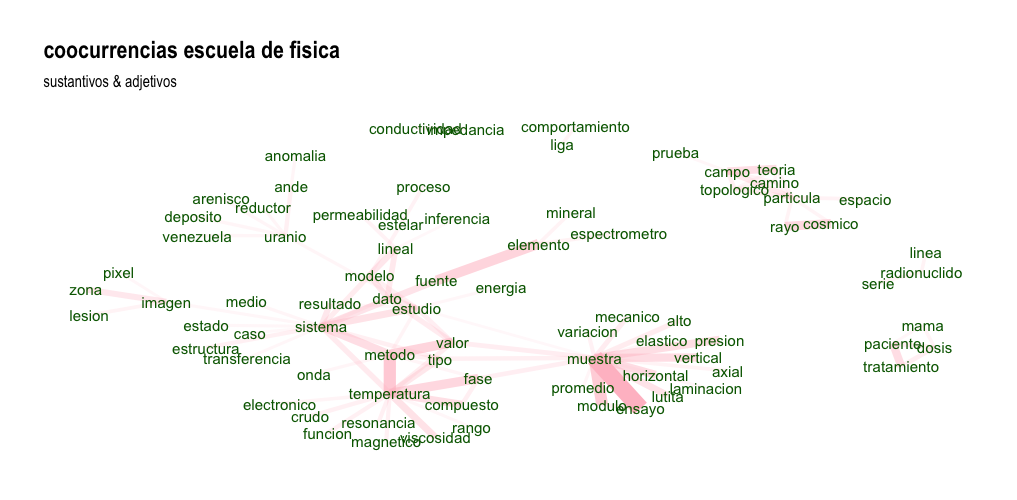
\includegraphics[width=0.9\linewidth]{images/03-marco-teorico/cooc} 

}

\caption{Coocurrencia de Palabras}\label{fig:coocejem}
\end{figure}

\hypertarget{similitud}{%
\section{Similitud de documentos:}\label{similitud}}

Para poder realizar la recomendación de documentos, una de las técnicas que se usa es medir la similitud que presenta un documento con los otros contenidos en el corpus. Un ejemplo de esta técnica es el uso de la similitud coseno que se explica con esta fórmula.

\begin{equation}
\cos ({\bf t},{\bf e})= {{\bf t} {\bf e} \over \|{\bf t}\| \|{\bf e}\|} = \frac{ \sum_{i=1}^{n}{{\bf t}_i{\bf e}_i} }{ \sqrt{\sum_{i=1}^{n}{({\bf t}_i)^2}} \sqrt{\sum_{i=1}^{n}{({\bf e}_i)^2}} }
\end{equation}

En la fórmula \emph{t} representa un documento y \emph{e} representa otro documento. Ambos documentos se asumen que están en un espacio con \emph{i} atributos, o dimensiones, y la intención es calcular un índice de similitud entre ambos documentos.

Este es uno de los métodos más usados para detectar similitudes en los textos, aunque existen otras fórmulas para el cálculo de la similitud como es el índice de jaccard.

El otro elemento de gran importancia en obtención de esta medición, es la representación que se haga del documento. Son distintas las técnicas que existen estando entre ellas la representación mediante ``bolsas de palabras'' o \emph{bag of words}. Recientemente se han creado formas más complejas para la representación como lo son los \emph{words embeddings} que son obtenidos mediante el entrenamiento de redes neuronales de aprendizaje profundo.

Estas formas de representación de textos serán investigadas más a fondo en futuras fases de la elaboración de este trabajo.

\hypertarget{sistemas-distribuidos}{%
\section{Sistemas Distribuidos:}\label{sistemas-distribuidos}}

Los distintos procesos y componentes de la Solución propuesta han sido diseñados e implementados como un sistema distribuido y por eso se hace la mención a este tema.

Una definición formal que se le puede dar a los sistemas distribuidos es ``cuando los componentes de hardware y/o sofware se encuentran localizados en una red de computadores y estos coordinan sus acciones sólo mediante el pase de mensajes'' \citep{distribu2012}.

Algunas de las principales características que tienen los sistemas distribuidos es la tolerancia a fallos, compartir recursos, concurrencia, ser escalables \citep{czaja2018} entre otras. Mencionamos estas en particular al ser propiedades que están presentes en la propuesta acá descrita.

\begin{enumerate}
\def\labelenumi{\arabic{enumi}.}
\item
  Fiabilidad o la llamada tolerancia a fallos: en caso de fallar un componente del sistema los otros se deben mantener en funcionamiento.
\item
  Compartir recursos: un conjunto de usuarios pueden compartir recursos como archivos o base de datos.
\item
  Concurrencia: poder ejecutar varios trabajos en simultáneo.
\item
  Escalable: al ser incrementada la escala del sistema se debe mantener en funcionamiento el sistema sin mayores contratiempos.
\end{enumerate}

\hypertarget{contenedores}{%
\subsection{Contenedores:}\label{contenedores}}

Un contenedor es una abstracción de una aplicación que se crea en un ambiente virtual, en el cual se encuentran ``empaquetados'' todos los componentes (sistema operativo, librerías, dependencias, etc.), que una aplicación necesita para poder ejecutarse. En su diseño se tiene presente que sean ligeros y que con otros contenedores pueden compartir el \emph{kernel}, usando un sistema de múltiples capas, que también pueden ser compartidas entre diversos contenedores, ahorrando espacio en disco del \emph{host} donde se alojan los contenedores.

El uso de los contenedores permite crear, distribuir y colocar en producción aplicaciones de software de una forma sencilla, segura y reproducible. También a cada contenedor se le puede realizar una asignación de recursos (memoria, cpu, almacenamiento) que garantice un óptimo funcionamiento de la aplicación que contienen.

Es importante señalar que el uso de esta tecnología añade un entorno de seguridad al estar cada contenedor en una ambiente isolado.

Para cada contenedor es necesario usar una imagen donde se definen las dependencias necesarias para su funcionamiento.

\hypertarget{orquestador}{%
\subsection{Orquestador:}\label{orquestador}}

Al tener diversos contenedores, donde cada uno aloja una aplicación distinta, puede resultar necesario que todos se integren en un sistema. Para que esta integración sea viable es necesario contar con un orquestador. Su uso permitirá lograr altos grados de portabilidad y reproducibilidad, pudiendo colocarlos en la nube o en centros de datos garantizando que se pueda hacer el \emph{deploy} de forma sencilla y fiel a lo que se implementó en el ambiente de desarrollo.

En el caso de la Solución propuesta se adoptará el uso de Docker Compose como orquestador y en el Capítulo que contiene la Propuesta Técnica \ref{propuestatec} serán expuestas las funcionalidades de cada contenedor y se apreciará la integración que brindará el orquestador.

\hypertarget{tendencias-actuales-sistemas-de-informaciuxf3n}{%
\section{Tendencias actuales Sistemas de Información:}\label{tendencias-actuales-sistemas-de-informaciuxf3n}}

Si bien anteriormente las búsquedas de información dentro de un conjunto de textos se procesaban determinando la aparición o no de palabras, o de frases dentro de un determinado texto, este método ha ido evolucionando para llegar hoy en día a un elevado nivel de abstracción, donde a partir de la necesidad de obtener una determinada información, es decir, de aquello que necesitamos buscar, que antes consistía en hacer \emph{match} con un objeto de información, se ha pasado de los motores de búsqueda ( \emph{search engines} ) a los motores de respuestas ( \emph{answering engines} ) \citep{balog2018}, donde el sistema ante un determinada consulta del usuario va a retornar una serie de resultados enriquecidos, mostrando la identificación de entidades, hechos y cualquier otro dato estructurado que esté de forma explícita, o incluso implícita, mencionado dentro de los textos que conforman el corpus.

Para lograr la generación de estos resultados se han tenido que conformar las llamadas bases de conocimiento o \emph{knowlodege bases}, que son repositorios donde previo a la búsqueda de la información dentro del sistema, se logra ir estructurando la organización de la información alrededor de objetos o datos específicos que se denominan \textbf{entidades}. Estos conceptos y métodos se asocian directamente a los que también se proponen, de manera más amplia, en la denominada \emph{web semántica} \footnote{Se basa en la idea de añadir \href{https://es.wikipedia.org/wiki/Metadato}{metadatos} \href{https://es.wikipedia.org/wiki/Sem\%C3\%A1ntica}{semánticos} y \href{https://es.wikipedia.org/wiki/Ontolog\%C3\%ADa_(Inform\%C3\%A1tica)}{ontológicos} a la \href{https://es.wikipedia.org/wiki/World_Wide_Web}{\emph{World Wide Web}}\emph{.} Esas informaciones adicionales ---que describen el contenido, el significado y la relación de los datos--- se deben proporcionar de manera formal, para que así sea posible evaluarlas automáticamente por máquinas de procesamiento. Tomado de \href{https://es.wikipedia.org/wiki/Web_sem\%C3\%A1ntica}{Wikipedia}} .

Como ejemplo de una \emph{knowledge bases} se puede mencionar a DBpedia, que se encuentra en la dirección \href{www.dbpedia.com}{www.www.dbpedia.org.com} y es un proyecto en donde puede acceder a una red global y unificada de grafos de conocimiento, la cual cubre más de 20 idiomas y principalmente genera sus grafos de conocimiento a partir de las publicaciones del Proyecto Wikipedia.

\hypertarget{temas-en-proceso-de-investigaciuxf3n}{%
\subsubsection{Temas en proceso de investigación:}\label{temas-en-proceso-de-investigaciuxf3n}}

Por estar aún en curso esta investigación a continuación se mencionan algunos temas que se está evaluando incluir en este marco teórico

\begin{itemize}
\item
  Métodos usados para el almacenamiento o la indexación como crear agrupamientos \emph{(clusters)} de aquellos documentos que compartan algunas características, por ejemplo, en la temática que aborden. Otra de las innovaciones que se están añadiendo a los sistemas de recuperación de información, es generar resúmenes con técnicas de procesamiento de lenguaje natural soportadas en el uso de arquitecturas de aprendizaje profundo \emph{(deep learning)} .
\item
  Resultados ante una búsqueda personalizados: al existir mecanismos como la sesión de usuario o las \emph{cookies} que guardan información contextual, permitiendo que ante un mismo \emph{query} en distintos equipos, los resultados sean distintos en función de la persona que hizo la búsqueda.
\item
  En cuanto al estado del arte existen distintas librerías y modelos de representación de documentos, palabras y caracteres. Algunos de estos modelos son fastext, word2vec, GPT3. Para este momento aún estamos haciendo la evaluación del uso de ellos para nuestra investigación, por lo cual, sólo los mencionamos referencialmente en este Anteproyecto.
\end{itemize}

\hypertarget{metodologuxeda}{%
\chapter{Marco Metodológico:}\label{metodologuxeda}}

\hypertarget{desarrollo}{%
\chapter{Desarrollo de la Solución:}\label{desarrollo}}

\hypertarget{conclusiones}{%
\chapter{Conclusiones:}\label{conclusiones}}

  \bibliography{references.bib}

\end{document}
